\documentclass[12pt,a4paper]{article}

% ─── Page Layout ───────────────────────────────────────────────────────────────
\usepackage[a4paper, margin=0.8in, headheight=14pt]{geometry}

% ─── Fonts (XeLaTeX) ───────────────────────────────────────────────────────────
\usepackage{fontspec}
\usepackage{unicode-math}
\setmainfont{TeX Gyre Pagella}
\setmonofont[Scale=0.88]{TeX Gyre Cursor}
\setmathfont{Latin Modern Math}

% ─── Packages ──────────────────────────────────────────────────────────────────
\usepackage{xcolor}
\usepackage{colortbl}
\usepackage{titlesec}
\usepackage{enumitem}
\usepackage{tabularx}
\usepackage{booktabs}
\usepackage{array}
\usepackage{amsmath}
\usepackage{tikz}
\usetikzlibrary{shapes.geometric, arrows.meta, positioning, calc, fit, decorations.pathreplacing}
\usepackage{tcolorbox}
\tcbuselibrary{skins, breakable}
\usepackage{hyperref}
\usepackage{fancyhdr}
\usepackage{graphicx}
\usepackage{microtype}
\hyphenpenalty=10000
\exhyphenpenalty=10000
\sloppy
\usepackage{caption}
\usepackage{setspace}
\usepackage{multirow}
\usepackage{tocloft}

% ─── Q&A helper ────────────────────────────────────────────────────────────────
\newcommand{\Q}[1]{\textbf{#1}\par\noindent\ignorespaces}

% ─── Colour Palette ────────────────────────────────────────────────────────────
\definecolor{myred}{RGB}{196,30,58}
\definecolor{mydark}{RGB}{30,30,50}
\definecolor{mygreen}{RGB}{14,120,80}
\definecolor{myteal}{RGB}{0,130,140}
\definecolor{myamber}{RGB}{180,100,0}
\definecolor{mypurple}{RGB}{100,30,160}
\definecolor{mygray}{RGB}{246,247,249}
\definecolor{mgframe}{RGB}{180,185,200}
\definecolor{watermark}{RGB}{145,150,170}
\definecolor{hdrred}{RGB}{250,232,235}
\definecolor{hdrgreen}{RGB}{220,244,233}
\definecolor{hdrteal}{RGB}{220,242,244}
\definecolor{hdramber}{RGB}{253,242,215}
\definecolor{hdrpurple}{RGB}{238,228,255}
\definecolor{hdrgray}{RGB}{238,240,245}
\definecolor{rowalt}{RGB}{250,251,253}

% ─── Section Formatting ────────────────────────────────────────────────────────
\titleformat{\section}
  {\large\bfseries\color{myred}}{\thesection.}{0.5em}{}
  [\vspace{1pt}{\color{myred}\rule{\linewidth}{0.8pt}}]
\titleformat{\subsection}
  {\normalsize\bfseries\color{myteal}}{\thesubsection}{0.5em}{}
\titlespacing*{\section}{0pt}{18pt}{7pt}
\titlespacing*{\subsection}{0pt}{11pt}{4pt}

% ─── Paragraph ─────────────────────────────────────────────────────────────────
\setlength{\parindent}{0pt}
\setlength{\parskip}{4pt}

% ─── TOC Styling ───────────────────────────────────────────────────────────────
\renewcommand{\cfttoctitlefont}{\large\bfseries\color{myred}}
\renewcommand{\cftaftertoctitle}{\par\noindent{\color{myred}\rule{\linewidth}{0.8pt}}}
\setlength{\cftbeforetoctitleskip}{0pt}
\setlength{\cftaftertoctitleskip}{6pt}
\renewcommand{\cftsecfont}{\normalsize\bfseries\color{mydark}}
\renewcommand{\cftsecpagefont}{\normalsize\bfseries\color{mydark}}
\renewcommand{\cftsecleader}{\cftdotfill{\cftdotsep}}
\setlength{\cftbeforesecskip}{7pt}
\renewcommand{\cftsubsecfont}{\small\color{mydark}}
\renewcommand{\cftsubsecpagefont}{\small\color{mydark}}
\setlength{\cftbeforesubsecskip}{3pt}
\setlength{\cftsubsecindent}{1.4em}

% ─── Table helpers ─────────────────────────────────────────────────────────────
\renewcommand{\arraystretch}{1.45}
\setlength{\tabcolsep}{6pt}
\arrayrulecolor{mydark}
\newcolumntype{B}[1]{>{\small\bfseries\raggedright\arraybackslash}m{#1}}
\newcolumntype{Y}{>{\small\raggedright\arraybackslash}X}
\renewcommand{\tabularxcolumn}[1]{m{#1}}

% ─── Header / Footer ───────────────────────────────────────────────────────────
\pagestyle{fancy}
\fancyhf{}
\fancyhead[L]{\small\color{myred}\textbf{PE-EC702A}\;\color{mydark}--- Adaptive Signal Processing}
\fancyhead[R]{\small\color{myteal}\textbf{Module 2 Notes}}
\fancyfoot[C]{\small\color{mydark}\thepage}
\fancyfoot[R]{\small\color{watermark}\textit{\copyright\ Biraj}}
\renewcommand{\headrulewidth}{0.5pt}
\renewcommand{\footrulewidth}{0.3pt}

% ─── Hyperref ──────────────────────────────────────────────────────────────────
\hypersetup{
  colorlinks=true, linkcolor=myteal, urlcolor=myteal,
  pdfauthor={Biraj Sarkar},
  pdftitle={PE-EC702A --- Module 2 Notes}
}

% ─── tcolorbox styles ──────────────────────────────────────────────────────────
\tcbset{
  tikzbox/.style={
    colback=mygray, colframe=mgframe, boxrule=0.6pt, arc=4pt,
    left=8pt, right=8pt, top=6pt, bottom=6pt,
    colbacktitle=mgframe, coltitle=mydark,
    fonttitle=\small\bfseries
  },
  defbox/.style={
    colback=hdrgreen, colframe=mygreen, boxrule=0.8pt, arc=4pt,
    left=9pt, right=9pt, top=6pt, bottom=6pt,
    colbacktitle=mygreen, coltitle=white,
    fonttitle=\small\bfseries
  },
  formulabox/.style={
    colback=hdrteal, colframe=myteal, boxrule=0.8pt, arc=4pt,
    left=9pt, right=9pt, top=7pt, bottom=7pt,
    colbacktitle=myteal, coltitle=white,
    fonttitle=\small\bfseries
  },
  examplebox/.style={
    colback=hdramber, colframe=myamber, boxrule=0.8pt, arc=4pt,
    left=9pt, right=9pt, top=6pt, bottom=6pt,
    colbacktitle=myamber, coltitle=white,
    fonttitle=\small\bfseries
  },
  masonbox/.style={
    colback=hdrpurple, colframe=mypurple, boxrule=0.8pt, arc=4pt,
    left=9pt, right=9pt, top=6pt, bottom=6pt,
    colbacktitle=mypurple, coltitle=white,
    fonttitle=\small\bfseries
  },
  exambox/.style={
    colback=hdrpurple, colframe=mypurple, boxrule=1pt, arc=5pt,
    left=10pt, right=10pt, top=8pt, bottom=8pt,
    colbacktitle=mypurple, coltitle=white,
    fonttitle=\bfseries,
    breakable, title after break={\textbf{Frequently Asked / Viva Questions (contd.)}}}
}
\tcbset{breakable}

% ─── TikZ styles ───────────────────────────────────────────────────────────────
\tikzset{
  block/.style={rectangle, draw=myteal, fill=hdrteal,
    text width=2.4cm, align=center, minimum height=0.95cm,
    font=\small, rounded corners=3pt, line width=0.7pt},
  redblock/.style={rectangle, draw=myred, fill=hdrred,
    text width=2.4cm, align=center, minimum height=0.95cm,
    font=\small, rounded corners=3pt, line width=0.7pt},
  netnode/.style={rectangle, draw=myteal, fill=hdrteal,
    text width=1.5cm, align=center, minimum height=0.8cm,
    font=\small, rounded corners=3pt, line width=0.7pt},
  sumjunc/.style={circle, draw=myamber, fill=hdramber,
    minimum size=0.62cm, font=\small, line width=0.8pt},
  snode/.style={circle, draw=mypurple, fill=hdrpurple,
    minimum size=0.55cm, font=\footnotesize, line width=0.7pt},
  arrow/.style={-Stealth, thick, color=mydark},
  redarrow/.style={-Stealth, thick, color=myred},
  line/.style={thick, color=mydark}
}

% ═══════════════════════════════════════════════════════════════════════════════
\begin{document}
% ═══════════════════════════════════════════════════════════════════════════════

\begin{center}
  {\LARGE\bfseries\color{myred} PE-EC702A --- Adaptive Signal Processing}\\[5pt]
  {\normalsize\color{mydark} Semester VII \quad$\bullet$\quad 3L:0T:0P \quad$\bullet$\quad 3 Credits}\\[3pt]
  {\normalsize\color{myteal}\textbf{Module 2 Exam Notes: Wiener Filters, Steepest Descent \& LMS}}\\[3pt]
  {\small\color{mydark} CGEC \;$|$\; B.Tech ECE (2023--27) \;$|$\; \textit{Biraj Sarkar}}
\end{center}
\vspace{2pt}
\noindent{\color{myred}\rule{\linewidth}{1.5pt}}
\vspace{2pt}

\hypersetup{linkcolor=mydark}
\tableofcontents
\hypersetup{linkcolor=myteal}
\newpage

% ===============================================================================
\section{Optimal FIR (Wiener) Filter}
% ===============================================================================

The Wiener filter is the optimal linear filter in the Mean-Square Error (MSE) sense. It assumes the signals are wide-sense stationary with known second-order statistics (autocorrelation and cross-correlation).

\subsection{Derivation of the Wiener-Hopf Equations}
Let the input vector be $\mathbf{x}(n) = [x(n), x(n-1), \dots, x(n-M+1)]^T$ and the weight vector be $\mathbf{w} = [w_0, w_1, \dots, w_{M-1}]^T$. The filter output is $y(n) = \mathbf{w}^H \mathbf{x}(n)$. The error signal is $e(n) = d(n) - y(n) = d(n) - \mathbf{w}^H \mathbf{x}(n)$.
The cost function to minimize is the Mean-Square Error $J(\mathbf{w}) = \mathbb{E}[|e(n)|^2]$:
\begin{equation}
  J(\mathbf{w}) = \mathbb{E}\left[(d(n) - \mathbf{w}^H \mathbf{x}(n))(d^*(n) - \mathbf{x}^H(n) \mathbf{w})\right]
\end{equation}
Expanding the expectation:
\begin{align}
  J(\mathbf{w}) &= \mathbb{E}[|d(n)|^2] - \mathbf{w}^H \mathbb{E}[\mathbf{x}(n) d^*(n)] - \mathbb{E}[d(n) \mathbf{x}^H(n)] \mathbf{w} + \mathbf{w}^H \mathbb{E}[\mathbf{x}(n) \mathbf{x}^H(n)] \mathbf{w} \nonumber \\
  &= \sigma_d^2 - \mathbf{w}^H \mathbf{p} - \mathbf{p}^H \mathbf{w} + \mathbf{w}^H \mathbf{R} \mathbf{w}
\end{align}
where $\sigma_d^2 = \mathbb{E}[|d(n)|^2]$, $\mathbf{p} = \mathbb{E}[\mathbf{x}(n) d^*(n)]$, and $\mathbf{R} = \mathbb{E}[\mathbf{x}(n) \mathbf{x}^H(n)]$.
To find the optimal weight vector $\mathbf{w}_o$, we differentiate $J(\mathbf{w})$ with respect to the complex conjugate of the weight vector $\mathbf{w}^*$ (or compute the gradient) and set it to zero:
\begin{equation}
  \nabla_{\mathbf{w}^*} J(\mathbf{w}) = -\mathbf{p} + \mathbf{R} \mathbf{w} = \mathbf{0}
\end{equation}
This yields the \textbf{Wiener-Hopf Equations}:
\begin{equation}
  \mathbf{R} \mathbf{w}_o = \mathbf{p} \implies \mathbf{w}_o = \mathbf{R}^{-1} \mathbf{p}
\end{equation}

\subsection{Minimum Mean-Square Error (\texorpdfstring{$J_{\text{min}}$}{Jmin})}
Substituting the optimal weight $\mathbf{w}_o$ back into the cost function $J(\mathbf{w})$ gives the minimum mean-square error:
\begin{equation}
  J_{\text{min}} = \sigma_d^2 - \mathbf{w}_o^H \mathbf{p} = \sigma_d^2 - \mathbf{p}^H \mathbf{R}^{-1} \mathbf{p}
\end{equation}

% ===============================================================================
\section{Method of Steepest Descent}
% ===============================================================================

When the statistics $\mathbf{R}$ and $\mathbf{p}$ are known, but inverting $\mathbf{R}$ is computationally expensive, we use the iterative Method of Steepest Descent. The weight vector is updated in the direction opposite to the gradient of the performance surface $J(\mathbf{w})$:

\subsection{Weight Update Equation}
\begin{equation}
  \mathbf{w}(n+1) = \mathbf{w}(n) - \frac{1}{2} \mu \nabla J(\mathbf{w}(n))
\end{equation}
where $\mu$ is the step-size parameter. Since $\nabla J(\mathbf{w}) = -2\mathbf{p} + 2\mathbf{R}\mathbf{w}(n)$, we have:
\begin{equation}
  \mathbf{w}(n+1) = \mathbf{w}(n) + \mu (\mathbf{p} - \mathbf{R} \mathbf{w}(n))
\end{equation}

\subsection{Convergence Analysis and Stability}
Let the weight error vector be defined as $\mathbf{c}(n) = \mathbf{w}(n) - \mathbf{w}_o$. Subtracting $\mathbf{w}_o$ from both sides of the update equation:
\begin{equation}
  \mathbf{c}(n+1) = (\mathbf{I} - \mu \mathbf{R})\mathbf{c}(n)
\end{equation}
Applying the spectral decomposition $\mathbf{R} = \mathbf{Q} \mathbf{\Lambda} \mathbf{Q}^H$ and defining the rotated error vector $\mathbf{v}(n) = \mathbf{Q}^H \mathbf{c}(n)$, we get:
\begin{equation}
  \mathbf{v}(n+1) = (\mathbf{I} - \mu \mathbf{\Lambda})\mathbf{v}(n)
\end{equation}
For stability, each decoupled mode $v_i(n+1) = (1 - \mu \lambda_i)v_i(n)$ must decay to zero, which requires $|1 - \mu \lambda_i| < 1$ for all $i$:
\begin{equation}
  0 < \mu < \frac{2}{\lambda_{\text{max}}}
\end{equation}
where $\lambda_{\text{max}}$ is the largest eigenvalue of the correlation matrix $\mathbf{R}$.

\begin{tcolorbox}[tikzbox, title={Contour Lines of MSE Surface and Convergence Trajectory}]
\centering
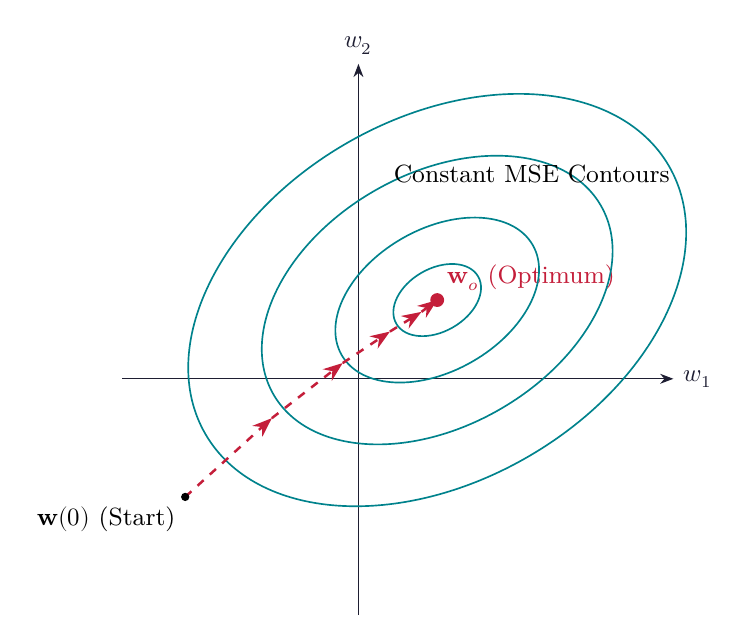
\begin{tikzpicture}[every node/.style={font=\small}]
  % Axes
  \draw[-Stealth, thin, color=mydark] (-3,0) -- (4,0) node[right] {$w_1$};
  \draw[-Stealth, thin, color=mydark] (0,-3) -- (0,4) node[above] {$w_2$};
  
  % Optimal Point
  \fill[color=myred] (1,1) circle (2.5pt) node[above right] {$\mathbf{w}_o$ (Optimum)};
  
  % Elliptical Contours
  \draw[color=myteal, semithick] (1,1) circle [x radius=0.6cm, y radius=0.4cm, rotate=30];
  \draw[color=myteal, semithick] (1,1) circle [x radius=1.4cm, y radius=0.9cm, rotate=30];
  \draw[color=myteal, semithick] (1,1) circle [x radius=2.4cm, y radius=1.6cm, rotate=30];
  \draw[color=myteal, semithick] (1,1) circle [x radius=3.4cm, y radius=2.3cm, rotate=30];
  
  % Trajectory path
  \draw[redarrow, dashed, line width=0.9pt] (-2.2,-1.5) -- (-1.1,-0.5);
  \draw[redarrow, dashed, line width=0.9pt] (-1.1,-0.5) -- (-0.2, 0.2);
  \draw[redarrow, dashed, line width=0.9pt] (-0.2, 0.2) -- (0.4, 0.6);
  \draw[redarrow, dashed, line width=0.9pt] (0.4, 0.6) -- (0.8, 0.85);
  \draw[redarrow, dashed, line width=0.9pt] (0.8, 0.85) -- (1.0, 1.0);
  
  \fill (-2.2,-1.5) circle (1.5pt) node[below left] {$\mathbf{w}(0)$ (Start)};
  \node at (2.2, 2.6) {Constant MSE Contours};
\end{tikzpicture}
\end{tcolorbox}

% ===============================================================================
\section{The Least Mean Squares (LMS) Algorithm}
% ===============================================================================

The Least Mean Squares (LMS) algorithm is a stochastic gradient descent algorithm. It avoids the need to know or estimate the ensemble statistics $\mathbf{R}$ and $\mathbf{p}$ by using instantaneous approximations:
\begin{equation}
  \hat{\mathbf{R}}(n) = \mathbf{x}(n) \mathbf{x}^H(n), \quad \hat{\mathbf{p}}(n) = \mathbf{x}(n) d^*(n)
\end{equation}

\subsection{LMS Algorithms Formulations}
The instantaneous cost function is chosen as $\hat{J}(n) = |e(n)|^2$. The update equations are:
\begin{tcolorbox}[defbox, title={LMS Update Equations}]
\textbf{Real-Valued LMS Algorithm:}
\begin{align}
  e(n) &= d(n) - \mathbf{w}^T(n) \mathbf{x}(n) \\
  \mathbf{w}(n+1) &= \mathbf{w}(n) + \mu e(n) \mathbf{x}(n)
\end{align}
\textbf{Complex-Valued LMS Algorithm:}
\begin{align}
  e(n) &= d(n) - \mathbf{w}^H(n) \mathbf{x}(n) \\
  \mathbf{w}(n+1) &= \mathbf{w}(n) + \mu \mathbf{x}(n) e^*(n)
\end{align}
\end{tcolorbox}

\subsection{LMS Convergence Analysis}
Under the \textbf{independence assumption} (the input vectors $\mathbf{x}(n)$ are statistically independent over time):
\begin{itemize}[leftmargin=*, itemsep=3pt]
  \item \textbf{Convergence in the Mean:} The ensemble average of the weights converges to the Wiener solution, $\mathbb{E}[\mathbf{w}(n)] \to \mathbf{w}_o$, if:
  \begin{equation}
    0 < \mu < \frac{2}{\lambda_{\text{max}}}
  \end{equation}
  A conservative practical limit based on total signal power is:
  \begin{equation}
    0 < \mu < \frac{2}{\text{Tr}(\mathbf{R})} = \frac{2}{M \cdot R_x(0)}
  \end{equation}
  \item \textbf{Convergence in the Mean-Square:} For the second-order statistics of the weights to remain stable, the step-size must satisfy:
  \begin{equation}
    0 < \mu < \frac{2}{\sum_{i=1}^M \lambda_i} = \frac{2}{\text{Tr}(\mathbf{R})}
  \end{equation}
\end{itemize}

\subsection{Excess MSE and Misadjustment}
Due to gradient estimation noise, the LMS algorithm does not settle exactly at $J_{\text{min}}$. It fluctuates about the optimum, introducing an \textbf{Excess Mean-Square Error} $J_{\text{ex}}$:
\begin{equation}
  J_{\text{ex}} = \lim_{n\to\infty} \mathbb{E}[|e(n)|^2] - J_{\text{min}}
\end{equation}
For a small step-size $\mu$, the excess MSE is given by:
\begin{equation}
  J_{\text{ex}} \approx \frac{\mu J_{\text{min}} \text{Tr}(\mathbf{R})}{2 - \mu \text{Tr}(\mathbf{R})}
\end{equation}
The \textbf{Misadjustment} $M$ is a dimensionless measure of how close the LMS filter is to the optimal Wiener filter:
\begin{equation}
  M = \frac{J_{\text{ex}}}{J_{\text{min}}} \approx \frac{\mu}{2} \text{Tr}(\mathbf{R}) = \frac{\mu}{2} \sum_{i=1}^M \lambda_i
\end{equation}

\begin{tcolorbox}[examplebox, title={Example: Wiener Filter Coefficient Design}]
A single-tap LMS filter has input signal $x(n)$ with variance $R_x(0) = 2$. The desired signal has variance $\sigma_d^2 = 5$, and the cross-correlation is $p = 1.6$. 
\begin{enumerate}[label=\textbf{\arabic*.}, leftmargin=*, itemsep=2pt]
  \item Determine the optimal weight $w_o$.
  \item Compute the minimum MSE $J_{\text{min}}$.
  \item Determine the maximum step-size $\mu$ for convergence in the mean.
  \item Calculate the misadjustment $M$ for $\mu = 0.05$.
\end{enumerate}

\textbf{Solution:}
\begin{enumerate}[label=\textbf{\arabic*.}, leftmargin=*, itemsep=4pt]
  \item Using the Wiener-Hopf equation:
    \[
      w_o = R^{-1}p = \frac{p}{R_x(0)} = \frac{1.6}{2} = 0.8
    \]
  \item The minimum MSE $J_{\text{min}}$ is:
    \[
      J_{\text{min}} = \sigma_d^2 - w_o p = 5 - (0.8 \times 1.6) = 5 - 1.28 = 3.72
    \]
  \item For a single-tap filter ($M=1$), $\lambda_{\text{max}} = R_x(0) = 2$. The step-size range is:
    \[
      0 < \mu < \frac{2}{\lambda_{\text{max}}} \implies 0 < \mu < 1
    \]
  \item The misadjustment $M$ for $\mu = 0.05$:
    \[
      M \approx \frac{\mu}{2} \text{Tr}(\mathbf{R}) = \frac{0.05}{2} \times 2 = 0.05 \text{ (or 5\%)}
    \]
\end{enumerate}
\end{tcolorbox}

% ===============================================================================
% MANDATORY QUICK REVISION PAGE
% ===============================================================================
\newpage
\begin{center}
  {\large\bfseries\color{myred} Quick Revision --- Module II}\\[3pt]
  {\small\color{mydark} Wiener Filters, Steepest Descent \& LMS $|$ PE-EC702A}
\end{center}
\noindent{\color{myred}\rule{\linewidth}{1.2pt}}
\vspace{4pt}

\begin{tcolorbox}[formulabox, title={\textbf{Key Formulas at a Glance}}]
\renewcommand{\arraystretch}{1.3}
\begin{tabularx}{\linewidth}{B{4.5cm} X}
Wiener-Hopf Equation & $\mathbf{R} \mathbf{w}_o = \mathbf{p} \implies \mathbf{w}_o = \mathbf{R}^{-1} \mathbf{p}$ \\[6pt]
Minimum MSE & $J_{\text{min}} = \sigma_d^2 - \mathbf{p}^H \mathbf{w}_o$ \\[6pt]
Steepest Descent Update & $\mathbf{w}(n+1) = \mathbf{w}(n) + \mu (\mathbf{p} - \mathbf{R}\mathbf{w}(n))$ \\[6pt]
LMS Update (Complex) & $\mathbf{w}(n+1) = \mathbf{w}(n) + \mu \mathbf{x}(n) e^*(n)$ \\[6pt]
Step-Size Bounds & $0 < \mu < \frac{2}{\lambda_{\text{max}}}$ \quad (Ensemble) or $0 < \mu < \frac{2}{\text{Tr}(\mathbf{R})}$ \quad (LMS) \\[6pt]
Misadjustment & $M = \frac{J_{\text{ex}}}{J_{\text{min}}} \approx \frac{\mu}{2} \text{Tr}(\mathbf{R})$
\end{tabularx}
\end{tcolorbox}

\begin{tcolorbox}[defbox, title={\textbf{One-Line Definitions}}]
\begin{itemize}[leftmargin=*, itemsep=2.5pt, topsep=0pt]
  \item \textbf{Wiener Filter:} The optimal linear time-invariant filter that minimizes mean-square error.
  \item \textbf{Steepest Descent:} An iterative optimization method that moves weights along the direction of maximum negative gradient.
  \item \textbf{LMS Algorithm:} A low-complexity adaptive algorithm using instantaneous signal values to approximate gradients.
  \item \textbf{Misadjustment:} A measure of the average excess MSE relative to the minimum MSE, representing algorithm noise.
  \item \textbf{Eigenvalue Spread:} The ratio $\lambda_{\text{max}}/\lambda_{\text{min}}$, indicating the convergence rate limit of gradient algorithms.
  \item \textbf{Independence Assumption:} An analytical simplification stating that successive tap-input vectors are statistically independent.
\end{itemize}
\end{tcolorbox}

\begin{tcolorbox}[exambox, title={\textbf{Frequently Asked / Viva Questions}}]
\begin{enumerate}[topsep=0pt, label=\textbf{Q\arabic*.}, itemsep=5pt]
  \item \Q{Derive the Wiener-Hopf equations for a real FIR filter.}
    See Section 1.1: We expand $J(\mathbf{w}) = \mathbb{E}[(d(n) - \mathbf{w}^T\mathbf{x}(n))^2] = \sigma_d^2 - 2\mathbf{w}^T\mathbf{p} + \mathbf{w}^T\mathbf{R}\mathbf{w}$. Differentiating w.r.t. $\mathbf{w}$ and setting to $\mathbf{0}$ yields $\mathbf{R}\mathbf{w}_o = \mathbf{p}$.
  \item \Q{What is the convergence criterion for the method of steepest descent?}
    The step-size parameter must satisfy $0 < \mu < 2/\lambda_{\text{max}}$, where $\lambda_{\text{max}}$ is the maximum eigenvalue of the autocorrelation matrix $\mathbf{R}$.
  \item \Q{Why is LMS referred to as a "stochastic" gradient algorithm?}
    Because it replaces the true gradient (which requires expectations of signals) with a noisy instantaneous gradient estimate computed directly from the current samples.
  \item \Q{Write down the complex LMS weight update equation and explain each term.}
    $\mathbf{w}(n+1) = \mathbf{w}(n) + \mu \mathbf{x}(n)e^*(n)$, where $\mathbf{w}(n)$ is the weight vector, $\mu$ is the step-size, $\mathbf{x}(n)$ is the input vector, and $e^*(n)$ is the complex conjugate of the error.
  \item \Q{What is the eigenvalue spread and how does it affect convergence speed?}
    Eigenvalue spread is the ratio $\chi = \lambda_{\text{max}}/\lambda_{\text{min}}$. A large eigenvalue spread (highly correlated input) causes the MSE surface to form a narrow valley, resulting in slow convergence.
  \item \Q{What is the physical meaning of misadjustment in LMS?}
    It represents the cost of adaptation; the weight vector continuously hunts around the optimum, causing the average MSE at steady state to be slightly larger than $J_{\text{min}}$.
  \item \Q{What is the conservative step-size limit used in practice for LMS?}
    $\mu < 2/\text{Tr}(\mathbf{R}) = 2/(M \cdot \text{Signal Power})$, which is easily calculated since it only requires the input signal power.
  \item \Q{Can the LMS algorithm converge if the step-size $\mu$ is negative?}
    No, if $\mu < 0$, the algorithm moves in the direction of the positive gradient, leading to divergence (instability) and weights going to infinity.
  \item \Q{How does the number of filter taps $M$ affect the misadjustment?}
    Since $M \approx \text{Tr}(\mathbf{R})/P_x$, a larger number of filter taps increases $\text{Tr}(\mathbf{R})$, which increases the misadjustment for a fixed step-size $\mu$.
  \item \Q{What is the minimum MSE ($J_{\text{min}}$) of a system where the input and desired signal are uncorrelated?}
    If they are uncorrelated, the cross-correlation vector $\mathbf{p} = \mathbf{0}$, giving $\mathbf{w}_o = \mathbf{0}$, which yields $J_{\text{min}} = \sigma_d^2$ (the total power of the desired signal).
\end{enumerate}
\end{tcolorbox}

\end{document}
